% ============================================================================
%  Chincol Artesanía — Guía de uso de las ilustraciones de fauna
%  Compilar desde esta carpeta:  pdflatex guia-fauna.tex  (dos veces, por el índice)
% ============================================================================
\documentclass[11pt,a4paper]{article}

\usepackage[utf8]{inputenc}
\usepackage[T1]{fontenc}
\usepackage[spanish,es-noshorthands]{babel}
\usepackage{tgpagella}
\usepackage{tgheros}
\usepackage[margin=2.3cm,top=2.6cm]{geometry}
\usepackage{graphicx}
\usepackage{xcolor}
\usepackage{tikz}
\usepackage{booktabs}
\usepackage{tabularx}
\usepackage{array}
\usepackage{enumitem}
\usepackage{listings}
\usepackage{tcolorbox}
\usepackage{fancyhdr}
\usepackage{titlesec}
\usepackage[hidelinks]{hyperref}

\graphicspath{{img/}}

% ---------- Paleta del sitio (src/app/globals.css) ----------
\definecolor{bg}{HTML}{F7F2EA}
\definecolor{sand}{HTML}{E6DACA}
\definecolor{ink}{HTML}{2B2019}
\definecolor{ink2}{HTML}{5A4A3C}
\definecolor{muted}{HTML}{6B5B4D}
\definecolor{accent}{HTML}{8A4B2A}
\definecolor{leather}{HTML}{3F2A1D}
\definecolor{gold}{HTML}{D6A77A}
\definecolor{line}{HTML}{E2D8C9}
\definecolor{fauna}{HTML}{D9C6A9}
\definecolor{faunaMovil}{HTML}{D6C3A7}
\definecolor{faunaOscuro}{HTML}{5A3F2F}

\color{ink}

% ---------- Títulos ----------
\titleformat{\section}{\Large\bfseries\color{accent}}{\thesection}{0.8em}{}
\titleformat{\subsection}{\large\bfseries\color{ink}}{\thesubsection}{0.7em}{}
\titlespacing*{\section}{0pt}{2.2ex}{1.2ex}

\setlength{\parindent}{0pt}
\setlength{\parskip}{0.7ex}
\setlist{itemsep=0.3ex,topsep=0.6ex}

% ---------- Encabezado ----------
\pagestyle{fancy}
\fancyhf{}
\fancyhead[L]{\small\sffamily\color{muted}Chincol Artesanía · Fauna del taller}
\fancyhead[R]{\small\sffamily\color{muted}\thepage}
\renewcommand{\headrulewidth}{0.4pt}
\renewcommand{\headrule}{\hbox to\headwidth{\color{line}\leaders\hrule height \headrulewidth\hfill}}

% ---------- Código ----------
\lstset{
  basicstyle=\ttfamily\small,
  backgroundcolor=\color{bg},
  frame=single, rulecolor=\color{line},
  framesep=6pt, xleftmargin=6pt, xrightmargin=6pt,
  keywordstyle=\color{accent}\bfseries,
  commentstyle=\color{muted}\itshape,
  stringstyle=\color{ink2},
  columns=fullflexible, keepspaces=true,
  breaklines=true, showstringspaces=false,
  literate={á}{{\'a}}1 {é}{{\'e}}1 {í}{{\'i}}1 {ó}{{\'o}}1 {ú}{{\'u}}1 {ñ}{{\~n}}1 {→}{{$\rightarrow$}}2 {…}{{...}}3,
}
\newcommand{\code}[1]{\texttt{\small #1}}

% ---------- Cajas ----------
\newtcolorbox{nota}[1][Nota]{colback=bg,colframe=gold,boxrule=0.6pt,arc=2pt,
  left=8pt,right=8pt,top=6pt,bottom=6pt,fonttitle=\sffamily\bfseries\small,
  coltitle=ink,colbacktitle=gold!35,title=#1}
\newtcolorbox{evitar}{colback=white,colframe=accent,boxrule=0.6pt,arc=2pt,
  left=8pt,right=8pt,top=6pt,bottom=6pt,fonttitle=\sffamily\bfseries\small,
  colbacktitle=accent,title=Evitar}

% Ficha de un animal en la galería
\newcommand{\ficha}[3]{%
  \begin{minipage}[t]{0.31\textwidth}\centering
    \includegraphics[width=\linewidth,height=3.2cm,keepaspectratio]{#1-tinta}\\[0.5ex]
    {\sffamily\bfseries #2}\\
    {\small\color{muted}\code{#1} · #3}
  \end{minipage}}

% ============================================================================
\begin{document}

% ---------- Portada ----------
\begin{titlepage}
  \pagecolor{bg}
  \centering
  \vspace*{1.2cm}
  {\sffamily\small\color{accent}\MakeUppercase{Taller de marroquinería}}\\[1.2ex]
  {\fontsize{34}{40}\selectfont\bfseries Fauna del taller}\\[1.5ex]
  {\Large\color{ink2}Guía de uso de las ilustraciones}\\[3ex]
  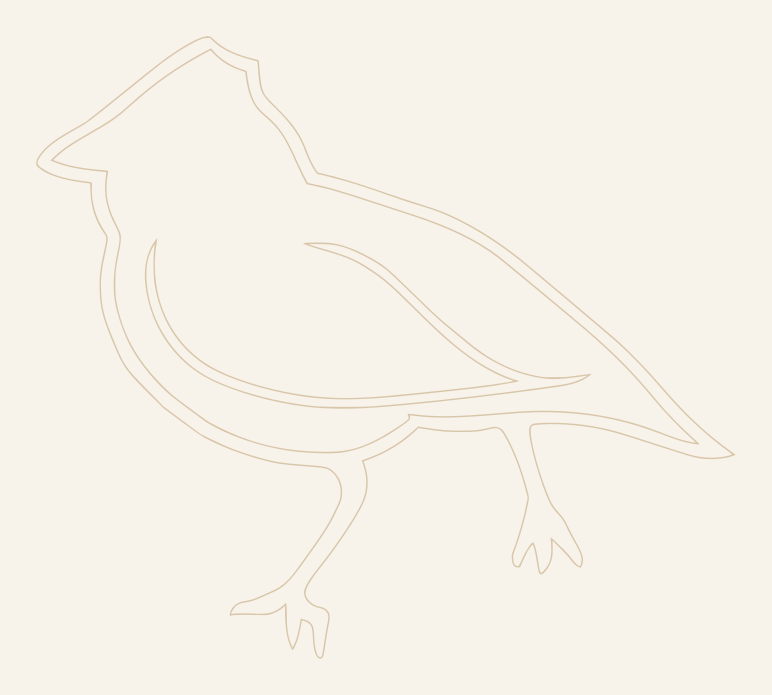
\includegraphics[width=0.52\textwidth]{chincol-claro}\\[1ex]
  \begin{tabular}{@{}c@{\hspace{0.6em}}c@{\hspace{0.6em}}c@{\hspace{0.6em}}c@{}}
    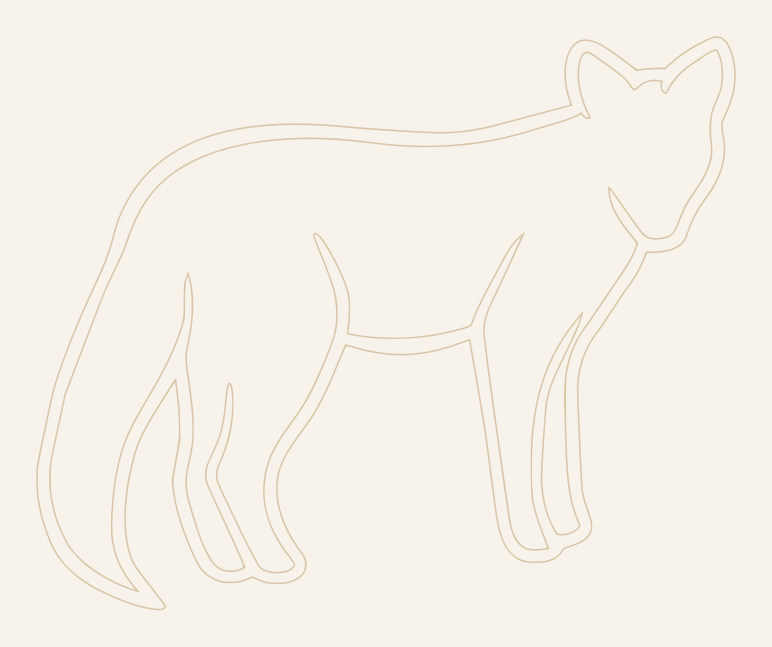
\includegraphics[height=2.1cm]{zorro-claro} &
    
\includegraphics[height=2.1cm]{pudu-claro} &
    
\includegraphics[height=2.1cm]{chinchilla-claro} &
    
\includegraphics[height=2.1cm]{fiu-claro}
  \end{tabular}
  \vfill
  {\sffamily\small\color{muted}
    Qué animales hay, dónde viven en la página y cómo moverlos, cambiarlos o agregar nuevos.\\
    Archivos: \code{src/components/PageAnimals.tsx} · \code{public/ilustraciones/} · \code{src/app/globals.css}}
\end{titlepage}
\nopagecolor

\tableofcontents
\vspace{2ex}

\begin{nota}[En resumen]
\begin{itemize}[leftmargin=1.2em]
  \item Los animales son \textbf{decoración de fondo}: van detrás del texto, no se pueden clicar y los lectores de pantalla los ignoran.
  \item Para \textbf{moverlos} o cambiarlos se edita \emph{una sola lista}: \code{ANIMALS} en \code{src/components/PageAnimals.tsx}.
  \item Toman el \textbf{color de la sección} donde están; el archivo SVG da solo la forma.
  \item Cada animal tiene una posición para \textbf{computador} y otra para \textbf{celular}.
\end{itemize}
\end{nota}

% ============================================================================
\section{Los cinco animales}

Todos son fauna nativa de Chile dibujada con la misma línea doble. El chincol es la marca; los demás acompañan.

\vspace{1ex}
\begin{center}
\ficha{chincol}{Chincol}{1532\,:\,1363}\hfill
\ficha{zorro}{Zorro}{1430\,:\,1174}\hfill
\ficha{pudu}{Pudú}{1494\,:\,1469}
\\[3ex]
\hspace*{0.17\textwidth}%
\ficha{chinchilla}{Chinchilla}{1263\,:\,814}\hspace{0.04\textwidth}%
\ficha{fiu}{Fiu-fiu}{1149\,:\,921}
\end{center}

\vspace{1ex}
Debajo de cada nombre va su \textbf{identificador} (el que se escribe en el código) y su \textbf{proporción} ancho\,:\,alto, que el sitio usa para que el dibujo nunca se deforme.

% ============================================================================
\section{Cómo funciona}

Son tres piezas, y en el día a día solo se toca la segunda:

\begin{center}
\begin{tikzpicture}[
  box/.style={draw=line,fill=white,rounded corners=2pt,minimum width=4.4cm,minimum height=1.9cm,align=center,font=\small},
  lab/.style={font=\sffamily\bfseries\small,text=accent},
  >=stealth]
  \node[box] (svg) at (0,0) {\code{public/ilustraciones/}\\\code{zorro.svg}, \code{pudu.svg}, …\\[0.3ex]{\color{muted}la \emph{forma}}};
  \node[box,draw=accent,line width=0.9pt] (lista) at (5.3,0) {\code{PageAnimals.tsx}\\lista \code{ANIMALS}\\[0.3ex]{\color{muted}\emph{dónde} y \emph{qué tamaño}}};
  \node[box] (css) at (10.6,0) {\code{globals.css}\\\code{.page-animals}\\[0.3ex]{\color{muted}el \emph{color} y la capa}};
  \node[lab,above=2pt of svg] {1 · Dibujo};
  \node[lab,above=2pt of lista] {2 · Ubicación (se edita aquí)};
  \node[lab,above=2pt of css] {3 · Estilo};
  \draw[->,color=muted] (svg) -- (lista);
  \draw[->,color=muted] (css) -- (lista);
\end{tikzpicture}
\end{center}

\begin{enumerate}
  \item \textbf{El dibujo.} Un SVG por animal en \code{public/ilustraciones/}. Se usa como \emph{máscara}: solo importa su silueta, no el color con que se exportó.
  \item \textbf{La ubicación.} La lista \code{ANIMALS} dice qué animal va en qué sección, en qué esquina y de qué tamaño.
  \item \textbf{El estilo.} En \code{globals.css} la clase \code{.page-animals} crea una capa invisible del tamaño de la sección, detrás del contenido, y le da el color por defecto.
\end{enumerate}

\subsection{Las secciones disponibles}

La página de inicio tiene cinco lugares preparados para recibir animales:

\begin{center}
\renewcommand{\arraystretch}{1.25}
\begin{tabularx}{0.92\textwidth}{@{}l X@{}}
\toprule
\textbf{Sección} & \textbf{Qué es en la página} \\
\midrule
\code{"hero"}     & Bloque de arriba, con el título y los botones. \\
\code{"piezas"}   & ``Piezas del taller'' (los productos destacados). \\
\code{"valores"}  & Franja blanca ``Cortado y cosido a mano…''. \\
\code{"encargos"} & Bloque oscuro ``¿Buscas algo que no está en el catálogo?''. \\
\code{"taller"}   & ``El taller'', al final de la página. \\
\bottomrule
\end{tabularx}
\end{center}

% ============================================================================
\section{Mover o cambiar un animal}

Abre \code{src/components/PageAnimals.tsx} y busca la lista \code{ANIMALS}. Cada línea es un animal:

\begin{lstlisting}
{ animal: "zorro", section: "piezas",
  desktop: { top: "36px", left: "38%", width: "150px", flip: true },
  mobile:  { top: "18px", right: "12px", width: "92px", flip: true } },
\end{lstlisting}

\subsection{Los campos}

\begin{center}
\renewcommand{\arraystretch}{1.25}
\begin{tabularx}{\textwidth}{@{}l X l@{}}
\toprule
\textbf{Campo} & \textbf{Para qué sirve} & \textbf{Ejemplo} \\
\midrule
\code{animal}  & Cuál dibujo. & \code{"pudu"} \\
\code{section} & En qué sección aparece. & \code{"taller"} \\
\code{desktop} & Posición y tamaño en computador (obligatorio). & ver abajo \\
\code{mobile}  & Posición en celular. Si no se pone, usa la de computador; con \code{null} no aparece en celular. & \code{null} \\
\code{color}   & Opcional: cambia el tono solo de ese animal. & \code{"\#c9b596"} \\
\midrule
\code{top} / \code{bottom} & Distancia al borde de arriba / de abajo de la sección. & \code{"40px"} \\
\code{left} / \code{right} & Distancia al borde izquierdo / derecho. & \code{"10\%"} \\
\code{width}   & Ancho del dibujo; el alto se calcula solo. & \code{"170px"} \\
\code{flip}    & \code{true} para que mire hacia el otro lado. & \code{true} \\
\bottomrule
\end{tabularx}
\end{center}

\subsection{Cómo se lee una posición}

Se usa \textbf{un} borde vertical (\code{top} \emph{o} \code{bottom}) y \textbf{un} borde horizontal (\code{left} \emph{o} \code{right}). Los valores pueden ser en \code{px} (fijos) o en \code{\%} del ancho o alto de la sección.

\begin{center}
\begin{tikzpicture}[>=stealth,font=\small]
  % sección
  \fill[bg] (0,0) rectangle (11,4.4);
  \draw[line,line width=0.8pt] (0,0) rectangle (11,4.4);
  \node[anchor=north west,font=\sffamily\bfseries\small,text=muted] at (0.15,4.3) {sección ``taller''};
  % texto de la sección
  \foreach \y in {3.2,2.8,2.4,2.0} \fill[line] (0.6,\y) rectangle (5.6,\y+0.16);
  % animal
  \node[anchor=north east,inner sep=0] (a) at (9.9,3.6) {
\includegraphics[width=2.4cm]{pudu-claro}};
  \draw[accent,dashed] (a.south west) rectangle (a.north east);
  % cotas
  \draw[<->,accent] (a.north east |- 0,4.4) -- node[right,text=accent]{\code{top: "40px"}} (a.north east);
  \draw[<->,accent] (a.north east) ++(0,-1.6) coordinate(p) (p) -- node[below,text=accent,yshift=-1pt]{\code{right: "10\%"}} (p -| 11,0);
  \draw[<->,accent] ([yshift=-8pt]a.south west) -- node[below,text=accent]{\code{width: "170px"}} ([yshift=-8pt]a.south east);
\end{tikzpicture}
\end{center}

\subsection{Recetas rápidas}

\begin{center}
\renewcommand{\arraystretch}{1.3}
\begin{tabularx}{\textwidth}{@{}X X@{}}
\toprule
\textbf{Quiero…} & \textbf{Cambio} \\
\midrule
Hacerlo más grande o más chico & Subir o bajar \code{width}. \\
Pegarlo a la esquina de abajo a la derecha & \code{bottom: "0px", right: "0px"} (y quitar \code{top}/\code{left}). \\
Que ``asome'' desde fuera del borde & Valores negativos: \code{bottom: "-24px"}. Lo que sobra se corta. \\
Que mire hacia el otro lado & \code{flip: true}. \\
Que no aparezca en celular & \code{mobile: null}. \\
Cambiarlo de sección & Cambiar \code{section}. \\
Quitarlo & Borrar su línea de la lista. \\
Poner otro animal en ese lugar & Cambiar \code{animal} (revisa \code{width}: cada dibujo tiene otra proporción). \\
\bottomrule
\end{tabularx}
\end{center}

\begin{center}
\begin{minipage}{0.3\textwidth}\centering
  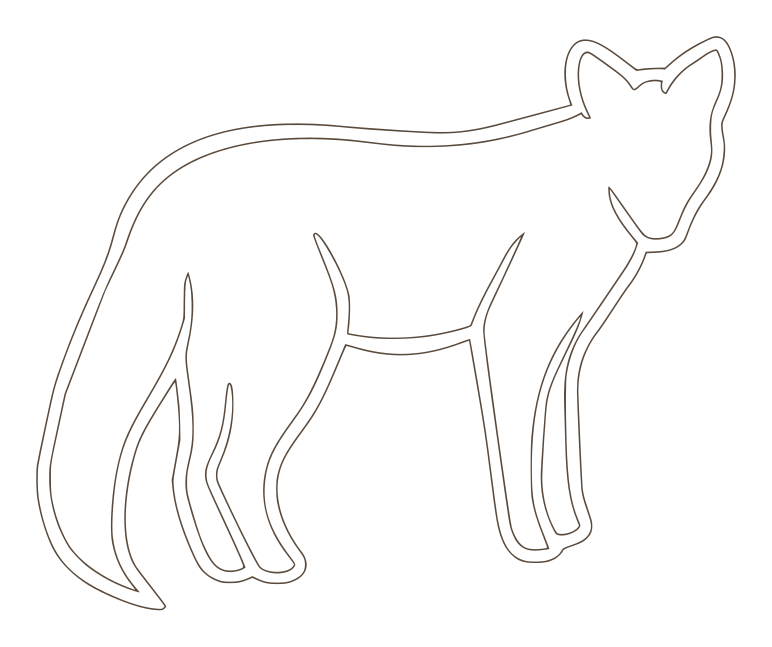
\includegraphics[width=0.85\linewidth]{zorro-tinta}\\{\small sin \code{flip}}
\end{minipage}
\begin{minipage}{0.3\textwidth}\centering
  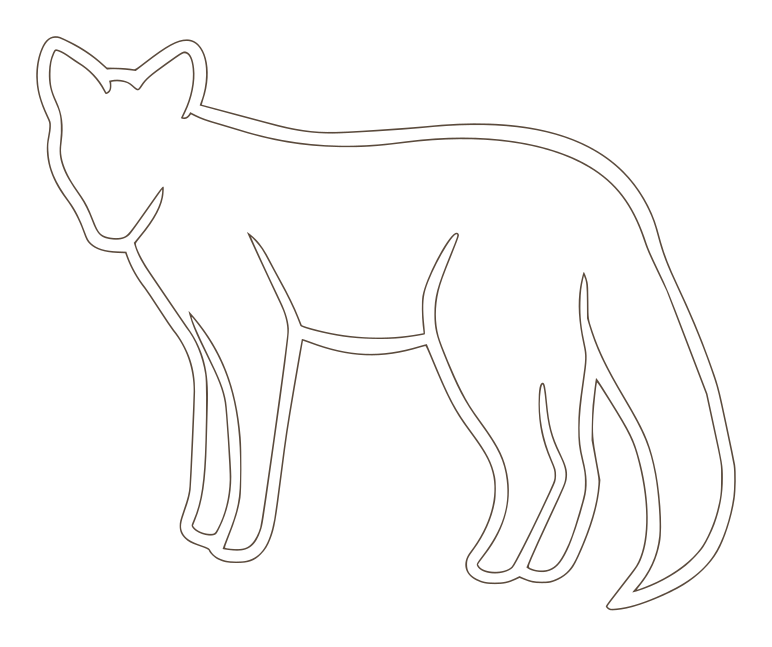
\includegraphics[width=0.85\linewidth]{zorro-tinta-flip}\\{\small \code{flip: true}}
\end{minipage}
\end{center}

% ============================================================================
\section{Computador y celular}

En pantallas de menos de \textbf{720\,px} de ancho cada animal usa su posición \code{mobile}. Hay tres opciones:

\begin{itemize}
  \item \textbf{Con \code{mobile: \{ … \}}}: usa esa posición y tamaño en celular. Es lo recomendado, porque en celular el espacio es menor y los animales deben ser más chicos (entre 70 y 140\,px).
  \item \textbf{Sin \code{mobile}}: repite la posición de computador. Úsalo solo si ya es pequeño y no tapa nada.
  \item \textbf{Con \code{mobile: null}}: el animal se oculta en celular.
\end{itemize}

\begin{nota}[Revisar siempre en los dos tamaños]
Después de mover un animal, mira la página en el computador y achica la ventana (o usa el modo celular del navegador, \code{F12} y luego el ícono de teléfono). Lo que se ve bien a 1440\,px puede quedar encima del título a 390\,px.
\end{nota}

% ============================================================================
\section{Color}

El SVG no define el color: el animal se pinta con el color de su sección. Así quedan siempre suaves y en el tono del sitio.

\begin{center}
\renewcommand{\arraystretch}{1.3}
\begin{tabular}{@{}c l l l@{}}
\toprule
& \textbf{Dónde} & \textbf{Color} & \textbf{Regla en \code{globals.css}} \\
\midrule
\tikz\fill[fauna,draw=line] (0,0) rectangle (0.5,0.35); & Secciones claras & \code{\#d9c6a9} & \code{.page-animals} \\
\tikz\fill[faunaMovil,draw=line] (0,0) rectangle (0.5,0.35); & Hero en celular (fondo arena) & \code{\#d6c3a7} & \code{.hero\_\_copy .page-animals} \\
\tikz\fill[faunaOscuro,draw=line] (0,0) rectangle (0.5,0.35); & Bloque oscuro ``encargos'' & \code{\#5a3f2f} & \code{.commission .page-animals} \\
\bottomrule
\end{tabular}
\end{center}

\begin{center}
\begin{minipage}{0.4\textwidth}\centering
  
\includegraphics[width=\linewidth]{fiu-claro}\\{\small sobre fondo claro}
\end{minipage}\hspace{0.05\textwidth}
\begin{minipage}{0.4\textwidth}\centering
  
\includegraphics[width=\linewidth]{fiu-oscuro}\\{\small sobre el bloque oscuro}
\end{minipage}
\end{center}

\begin{itemize}
  \item Para cambiar el tono de \textbf{todos} los animales de un tipo de fondo, edita el color en la regla de \code{globals.css}.
  \item Para cambiar \textbf{uno solo}, agrega \code{color: "\#…"} a su línea en \code{ANIMALS}.
  \item La idea es que se \emph{adivinen}, no que compitan con el texto: un tono apenas más oscuro (o más claro, en fondo oscuro) que el fondo.
\end{itemize}

% ============================================================================
\section{Cómo está hoy la página}

Ubicación actual según la lista \code{ANIMALS}:

\begin{center}
\renewcommand{\arraystretch}{1.3}
\begin{tabularx}{\textwidth}{@{}c l X X@{}}
\toprule
& \textbf{Animal} & \textbf{Computador} & \textbf{Celular} \\
\midrule

\includegraphics[height=0.8cm]{chinchilla-tinta} & Chinchilla · \code{hero} & arriba, al centro (\code{left: 44\%}), 118\,px & arriba a la izquierda, 72\,px \\
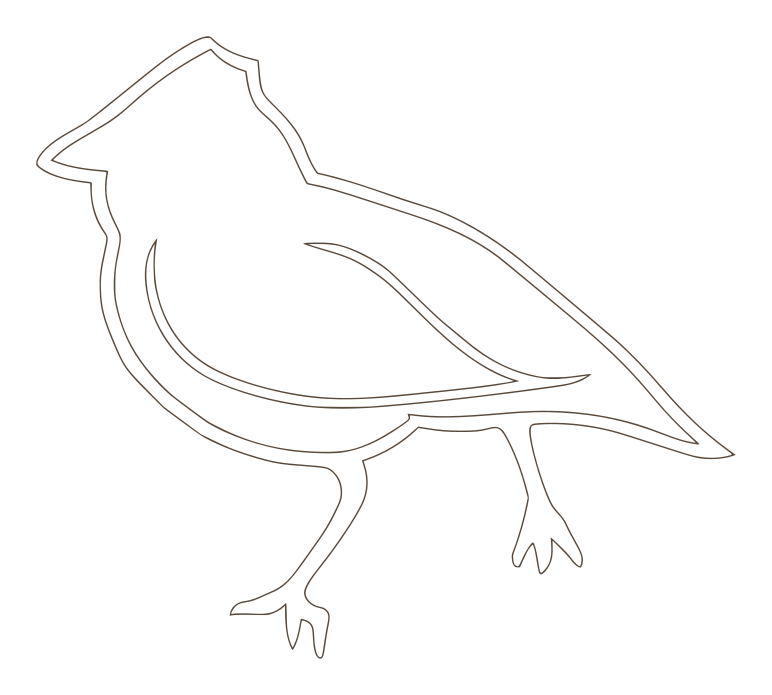
\includegraphics[height=0.8cm]{chincol-tinta} & Chincol · \code{hero} & abajo a la derecha, asomando, 250\,px & arriba a la derecha, 112\,px \\
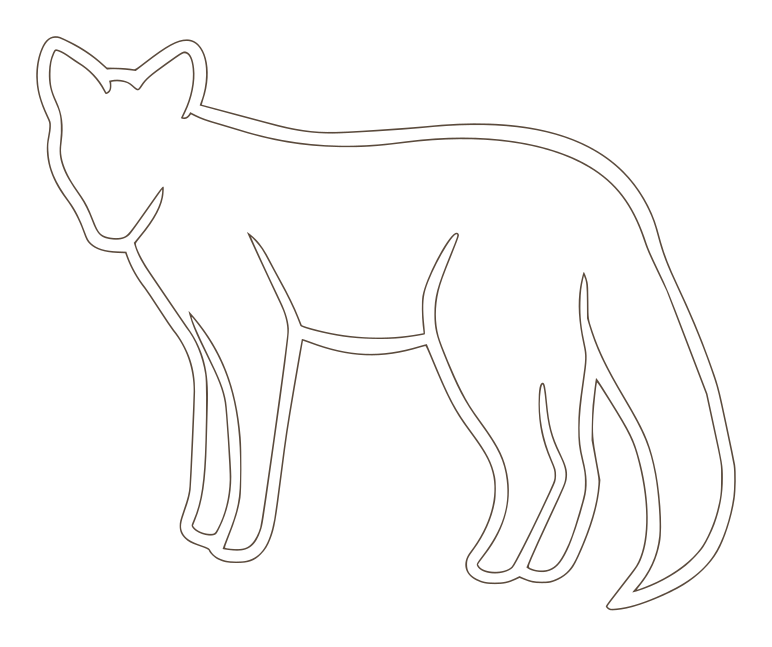
\includegraphics[height=0.8cm]{zorro-tinta-flip} & Zorro · \code{piezas} & arriba, al centro (\code{left: 38\%}), 150\,px, volteado & arriba a la derecha, 92\,px \\
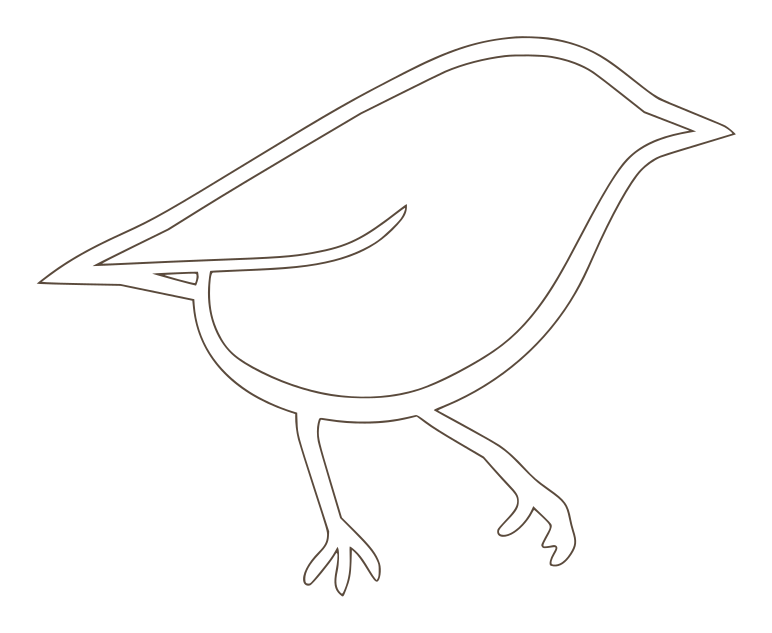
\includegraphics[height=0.8cm]{fiu-tinta} & Fiu-fiu · \code{encargos} & abajo a la derecha, asomando, 220\,px & abajo a la derecha, 140\,px \\
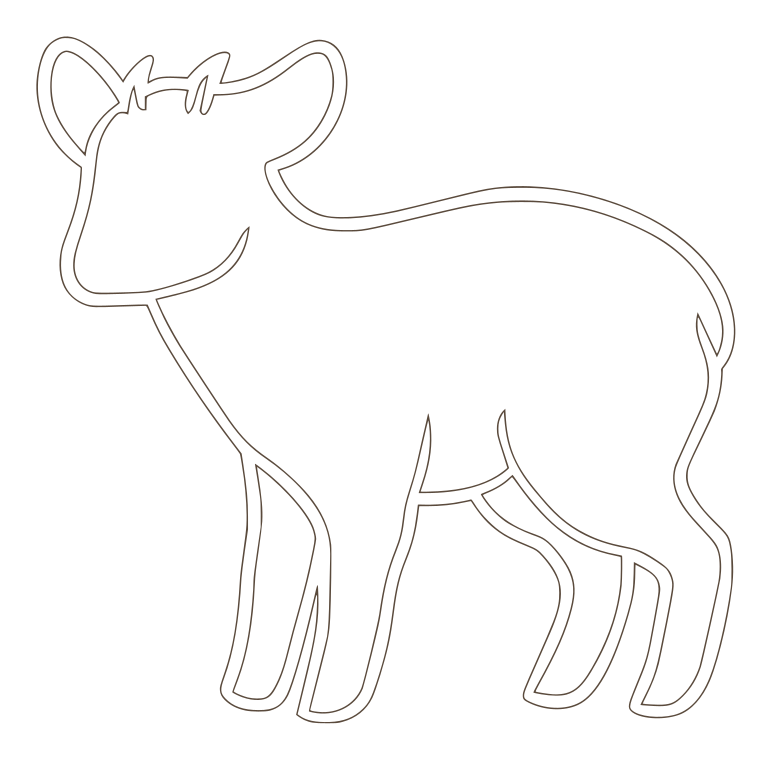
\includegraphics[height=0.8cm]{pudu-tinta} & Pudú · \code{taller} & arriba a la derecha (\code{right: 10\%}), 170\,px & arriba a la derecha, 96\,px \\
\bottomrule
\end{tabularx}
\end{center}

La sección \code{"valores"} está preparada pero hoy no tiene ningún animal.

% ============================================================================
\section{Agregar un animal nuevo}

\subsection{1. Preparar el dibujo}

\begin{itemize}
  \item Exportar como \textbf{SVG} desde Illustrator (\emph{Archivo → Exportar → Exportar como… → SVG}).
  \item \textbf{Borrar u ocultar la imagen de referencia} antes de exportar. Si queda dentro, el archivo pesa megas en vez de kilobytes (los actuales pesan entre 8 y 19\,KB).
  \item Un solo color de relleno, sin fondo. El color da igual: el sitio lo reemplaza.
  \item Recortar la mesa de trabajo al dibujo (\emph{Objeto → Mesas de trabajo → Ajustar a los límites del arte}), para que no quede espacio vacío alrededor.
  \item Nombre en minúsculas, sin tildes ni espacios: \code{huemul.svg}, \code{picaflor.svg}.
\end{itemize}

\subsection{2. Registrarlo}

\begin{enumerate}
  \item Copiar el archivo a \code{public/ilustraciones/}.
  \item En \code{PageAnimals.tsx}, agregar el nombre al tipo \code{Animal}:
\begin{lstlisting}
type Animal = "chincol" | "zorro" | "pudu" | "chinchilla" | "fiu" | "huemul";
\end{lstlisting}
  \item Agregar su proporción en \code{ASPECT}. Son los dos últimos números del \code{viewBox} del SVG (ábrelo con un editor de texto; está en la primera línea):
\begin{lstlisting}
// <svg ... viewBox="0 0 1210 980">   →   ancho 1210, alto 980
huemul: "1210 / 980",
\end{lstlisting}
  \item Ubicarlo con una línea nueva en \code{ANIMALS}, como en la sección 3.
\end{enumerate}

\subsection{Agregar animales en otra sección o página}

Una sección nueva necesita dos cosas en su HTML: la clase \code{has-animals} en el contenedor y el componente dentro:

\begin{lstlisting}
<section className="section container has-animals">
  <PageAnimals section="catalogo" full />
  ...
</section>
\end{lstlisting}

y agregar \code{"catalogo"} al tipo \code{Section}. La opción \code{full} se usa cuando la sección tiene la clase \code{container}, para que el animal pueda ir hasta el borde de la pantalla y no solo hasta el borde de la columna de texto.

% ============================================================================
\section{Buenas prácticas}

\begin{itemize}
  \item \textbf{Uno, a lo más dos, por sección.} Son un guiño, no un patrón de fondo.
  \item \textbf{En los márgenes y esquinas}, lejos de títulos, precios y botones.
  \item \textbf{Variar el animal} entre secciones seguidas; el chincol se reserva para el inicio y la marca.
  \item \textbf{Asomar desde el borde} (valores negativos) queda más natural que un animal flotando al medio.
  \item \textbf{Tamaños de referencia:} 110--260\,px en computador, 70--140\,px en celular.
\end{itemize}

\vspace{1ex}
\begin{evitar}
\begin{itemize}[leftmargin=1.2em]
  \item Ponerlos encima del texto o de las fotos de producto: se pierden y ensucian la lectura.
  \item Usar colores fuertes (el acento, negro): dejan de ser fondo.
  \item Exportar el SVG con la imagen de referencia incrustada.
  \item Cambiar \code{width} en computador y olvidar el de \code{mobile}.
  \item Poner el mismo animal dos veces en la misma sección: el código los distingue por nombre y se confunden.
\end{itemize}
\end{evitar}

\end{document}
